\inputencoding{utf8}
\chapter[Testiranje zmogljivosti Amazon EC2 platforme (P. Matičič, J. Pelicon, B. Rojc)]{Testiranje zmogljivosti Amazon EC2 platforme}

\pagestyle{fancy}
\fancyhf{}
\fancyhead[LE,RO]{\thepage}
\fancyhead[RE,LO]{\leftmark}

\huge Peter Matičič, Jan Pelicon, Blaž Rojc
\normalsize
\bigskip

\section{Opis problema}

%Z dneva v dan proizvedemo čedalje več slik.
%Predstavljajo znaten delež podatkov, shranjenih v raznih storitvah v oblaku.
%Ampak ko želimo najti določen predmet ali osebo, ki smo jo slikali, je ročno brskanje po digitalnih zbirkah zamudno.
%
%S tem problemom v mislih bomo stestirali oblačno platformo Amazon EC2.
%Ustvarili bomo enostavno storitev, ki bo uporabniku omogočala iskanje vzorcev v večjem naboru slik, shranjenih v oblaku.
%Poglobili se bomo v zahtevnost uporabe za programerja, fleksibilnost pri programiranju in morebitnem prenašanju storitve na druge platforme,
%	odzivnost in izkušnjo za uporabnika ter zmogljivost in skalabilnost virov na platformi.

Med programerji je veliko takšnih, ki sanjajo o tem, bi bili naslednji Bill Gates, Mark Zuckerberg ali Steve Jobs.
Imajo idejo, za katero verjamejo, da bo zavzela svet in jim prinesla miljone ter večno slavo.
Ampak potrebujejo platformo, na kateri bo njihova storitev tekla.
En sam prenosnik ne more vendar streči tisočem uporabnikom s celega sveta hkrati.
Platforma mora biti cenovno dostopna, hkrati pa tudi poljubno razširljiva, da, ko se zgodi neizogiben naval uporabnikov, lahko programer enostavno in hitro aktivira dodatno procesno moč.

Tu vstopi Amazonov Elastic Cloud. %\cite{1_aws_ec_site} % https://aws.amazon.com/
Obljublja dostopne cene, fleksibilno alokacijo računskih virov in za nadobudnega podjetnika najpomembneje možnost uporabe določenih storitev brezplačno.
Med temi storitvami je na voljo tudi najem tako imenovanih ``mikro instanc''. %\cite{1_aws_free} % https://aws.amazon.com/free/
To so virtualni spletni strežniki z enim procesnim jedrom in 1 GB pomnilnika.
Predstavljajo minimalno konfiguracijo, ki lahko gosti poljubno spletno storitev.
Hkrati pa predstavlja procesno ozko grlo, katerega omejitve moramo upoštevati pri tvorbi storitve.

S tem v mislih želimo stestirati platformo Amazon EC2.
Ustvarili bomo enostavno storitev, ki bo uporabniku omogočala iskanje vzorcev v večjem naboru slik, shranjenih v oblaku.
Predstavljala bo generično spletno aplikacijo, ki potrebuje ravno dovolj računske moči, da se bodo pojavile slabosti mikro instanc, v obliki upočasnjenega ali onemogočenega delovanja na strani uporabnika.
Osnova storitve je iskanje vzorca v naboru slik.
Uporabnik od storitve zahteva podatek o tem, v katerih slikah se ta vzorec nahaja, pričakuje pa hiter odgovor, ne več kot nekaj sekund zamika.
Taka storitev nam bo omogočala relativno enostavno merjenje odzivnosti platforme, modularnost nalaganja kode in morebitno razširljivost v primeru večjega števila hkratnih uporabnikov.

\section{Realizacija}

\subsection{Aplikacija}

\begin{figure}[H]
\centering
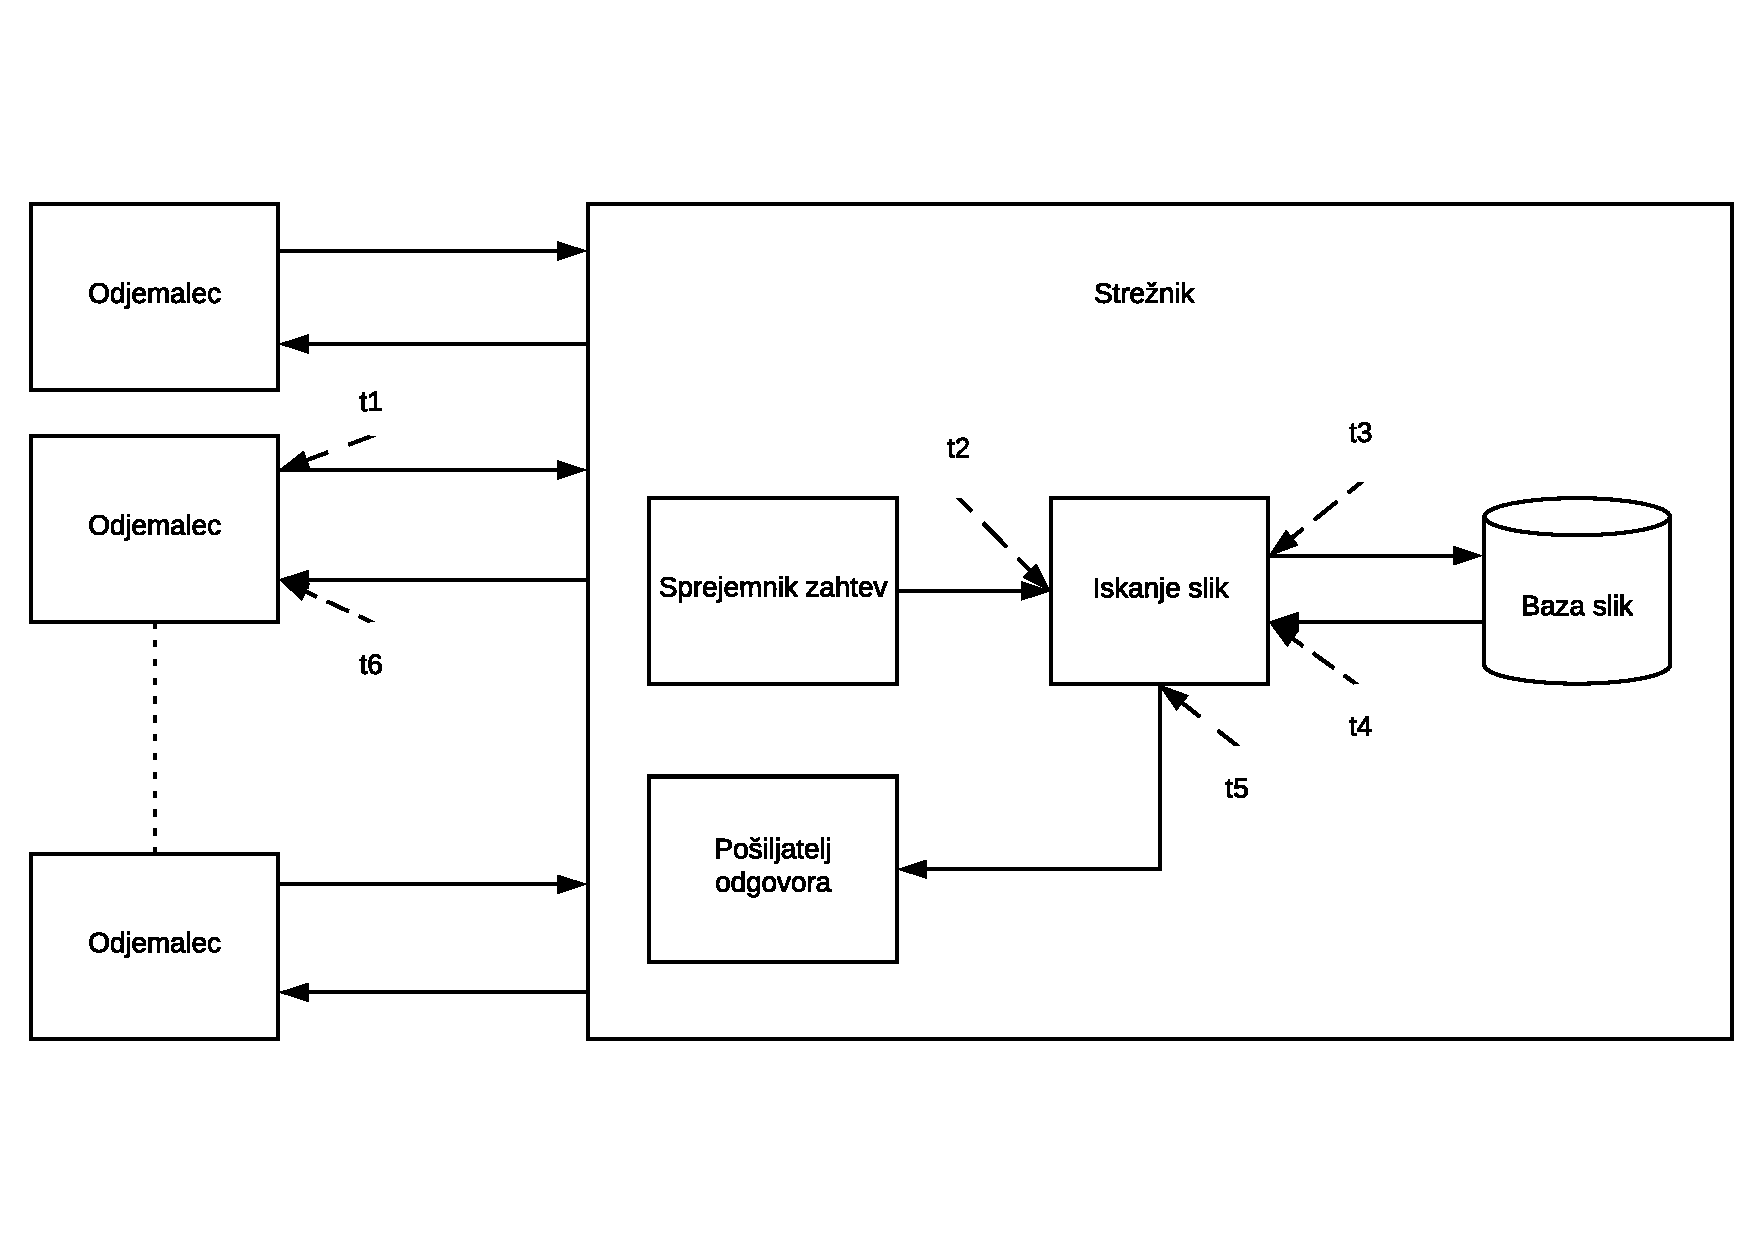
\includegraphics[scale=0.4]{Img/1_shema.pdf}
\caption{Shema aplikacije.}
\label{fig:1_osnovnaShema}
\end{figure}

Aplikacija je realizirana kot spletna storitev, t.j. strežnik, dostopen na spletu, ki se odziva na zahteve uporabnikov.
Uporabnik strežniku pošlje zahtevo v obliki JSON niza, ki vsebuje zaporedno številko zahteve, podatek o tipu zahteve in potrebne parametre.
Strežnik zahtevo primerno obdela in vrne rezultat v obliki JSON niza, katerega oblika je odvisna od tipa zahteve.

\subsection{Tipi zahtev}

V osnovi vsi tipi zahtev vključujejo iskanje vzorca v naboru slik.
Razlikujejo se v tipu vzorca, ki ga uporabnik želi najti v sliki.
Storitev nudi tri tipe iskanj: iskanje specifične barve piksla, iskanje vzorca s prosojnostno masko in iskanje slikovnega izseka.

\subsubsection{Iskanje specifične barve piksla}

Storitev prejme podatek o iskani barvi piksla, preišče vsako sliko in vrne prvo pojavitev iskanega piksla.

\subsubsection{Iskanje vzorca s prosojnostno masko}

Storitev prejme slikovni izsek in pripadajočo prosojnostno masko.
Med slikami najde lokacijo, ki se z izsekom najbolje ujema, in jo vrne uporabniku.

\subsubsection{Iskanje slikovnega izseka}

Storitev prejme slikovni izsek.
Preišče slike in, ko najde prvo ujemanje, rezultat vrne uporabniku.

\subsection{Amazon Web Services (AWS)}

Za delo z Amazon Web Services si mora uporabnik ustvariti račun v njihovem sistemu. Po uspešni registraciji si lahko ustvarimo svojo instanco EC2 storitve, ki nam jo Amazon ponuja zastonj za eno leto pri čemer na mesec porabimo največ 750 ur delovanja. Obsežnejša navodila so na voljo tudi na Amazonovi spletni strani \cite{1_aws_ec2_tutorial}, mi pa smo to naredili tako, da se postavimo v AWS Management Console, kjer lahko izberemo opcijo \emph{Launch a virtual machine with EC2}. Takoj nam konzola ponudi izbiro slike, katero bi uporabljali na novi virtualki kot prikazano na sliki \ref{fig:1_AWS_images}. Za naš projekt smo izbrali sliko Amazon Linux 2 AMI c.

\begin{figure}[H]
    \centering
    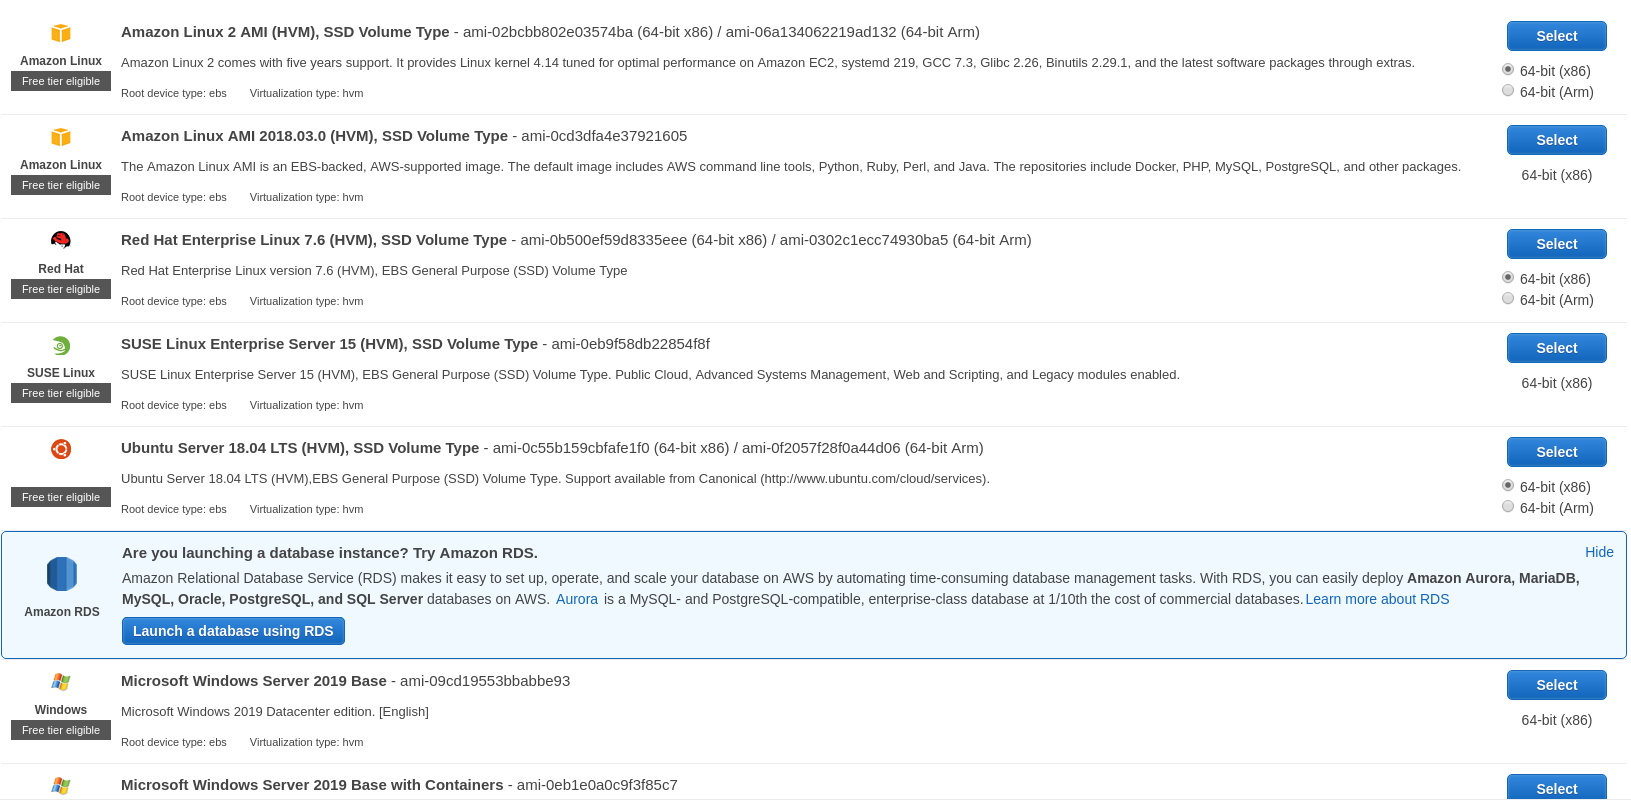
\includegraphics[scale=0.25]{Img/1_AWS_images.png}
    \caption{Slike za izdelavo virtualke}
    \label{fig:1_AWS_images}
\end{figure}

V naslednjem koraku izberemo tip instance slike, to je Amazonov način izbire paketov, ki vključujejo različne funkcionalnosti. V našem primeru ker izbiramo brezplačno različico, nam ponujajo tip t2.micro, ki vsebuje 1 jedro, 1GB pomnilnika, samo začasno hranjenje podatkov na disku in nižjo hitrost povezave. Za tem lahko nadaljujemo z nastavljanjem različnih konfiguracij naše virtualke ali pa preprosto kliknemo Review and Launch, ki nam ponudi še en pregled čez izbrane nastavitve in zažene virtualko. Po zagonu virtualke nam sistem ponudi opcijo generiranja para ključev za varno SSH povezavo do nje. Ko zaključimo z ustvarjanjem, se premaknemo v EC2 management console kjer kliknemo na \emph{instances}. Od tam lahko opazujemo status naše storitve in pridobimo tudi naslov, na katerem se nahaja. Za povezavo uporabimo javni naslov storitve, uporabnika $ec2-suser$ za varnost pa uporabimo $.pem$ datoteko, ki smo jo v prejšnjem koraku prenesli. Ko se uspešno povežemo na storitev, lahko pričnemo z razvojem naše aplikacije.

\subsection{Aplikacija}

Aplikacija je napisana v programskem jeziku Java. Sestavljata jo odjemalska in strežniška komponenta, ki uporabljata skupne enumeratorje za določanje tipa zahteve. Zahteve sestavlja odjemalec in jih pošlje strežniku, ki to zahtevo obdela - začne iskanje v slikah in pripravi prvi najden rezultat. Povezava med strežnikom in odjemalcem je trajna, dokler je eden od njiju ne prekine, kar nam omogoči, da pri meritvah ne upoštevamo časa vzpostavitve povezave. Podatki se prenašajo v obliki JSON, ki vsebuje sekvenčno številko zahteve, tip zahteve in morebitne dodatne podatke, ki so potrebni za obdelavo. Strežnik ob prejemu podatkov začne z delom na ustrezni zahtevi ter nato pošlje odgovor klientu z številko zahteve in rezultatom. Strežniški del je napisan tako, da lahko paralelno obdeluje več zahtev.

\section{Predvidevanje metrik}

Kot glavno metriko bomo opazovali skupni čas zahteve in odgovora.
Podrobneje ga bomo razdelili na čas potovanja zahteve od nas do strežnika ($t_2 - t_1$), čas obdelave na strežniku ($t_3 - t_2$) in čas potovanja odgovora od strežnika do nas ($t_4 - t_3$) (časi označeni na sliki \ref{fig:1_osnovnaShema}).
Zanima nas, kako se sistem odziva na zahteve ob različnih urah in kako se časi odgovorov podaljšajo glede na število hkratnih uporabnikov.

\section{Rezultati meritev}

\section{Plan dela}

\begin{itemize}
\item implementacija iskalnih algoritmov (1 / 3 narejenih)
\item določitev bremen - čas meritev, število hkratnih uporabnikov, ... ?
\item določitev metrik 
\item določitev orodij - avtomatizacija merjenja, zbiranje rezultatov
\end{itemize}

\section{Literatura}

%\bibliographystyle{ieeetr}
%\bibliography{poglavje_1}

\inputencoding{cp1250}